\videotitle{Blackbox Optimization Methods}

%--------------------------------------------g-----


\myframe{NAS as Hyperparameter Optimization}{
	\myit{
		\item \alert{NAS can be formulated as a HPO problem}
	}
\medskip
\pause

\begin{columns}[T]
\column{0.00\textwidth}
\column{0.73\textwidth}
	\myit{
		\item E.g., cell search space by \lit{\href{https://openaccess.thecvf.com/content_cvpr_2018/papers/Zoph_Learning_Transferable_Architectures_CVPR_2018_paper.pdf}{Zoph et al. 2018}} \\ has 5 categorical choices per block
		
		\myit{
			\item 2 categorical choices of hidden states
			\myit{
				\item For block $N$, the domain of these categorical variables is $\{h_i, h_{i-1}, \text{output of block } 1, ..., \text{output of block } N-1\}$
			}
			\item 2 categorical variables choosing between operations
			\item 1 categorical variable choosing the combination method
			\item Total number of hyperparameters for the cell: \\ 5B (with B=5 by default)
		}
	}
\column{0.27\textwidth}
	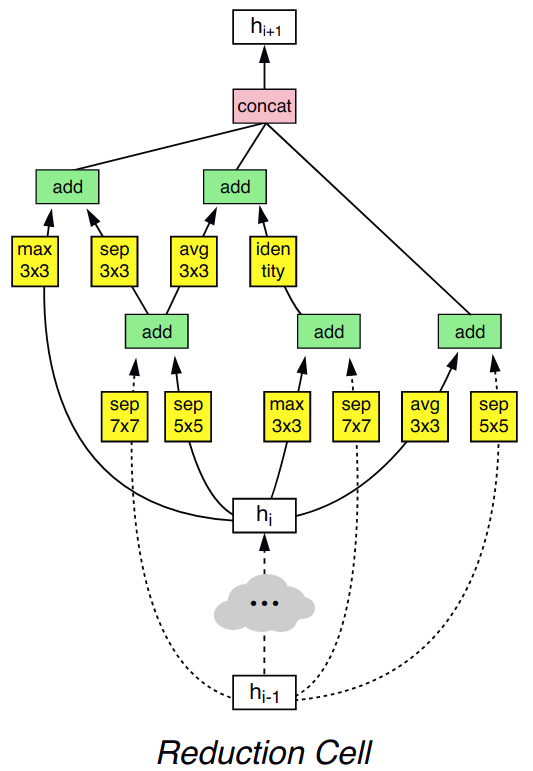
\includegraphics[width=\textwidth]{images/nasnet_reduce.png}
\end{columns}

\pause
\vspace*{-1.5cm}
	\myit{
		\item \alert{In general: one may require conditional hyperparameters}
		\myit{
			\item E.g., chain-structured search space
			\myit{
				\item Top-level hyperparameter: number of layers L
				\item Hyperparameters of layer k conditional on L $\ge$ k
			}
		}
		
	}
}
%-----------------------------------------------------------------------





\myframe{Early Work on Neuroevolution (already since the 1990s)\\ \litw{\href{https://content.wolfram.com/uploads/sites/13/2018/02/04-4-6.pdf}{Kitano. 1990}; \href{http://www.demo.cs.brandeis.edu/papers/ieeenn.pdf}{Angeline et al. 1994}; \href{http://nn.cs.utexas.edu/downloads/papers/stanley.ec02.pdf}{Stanley and Miikkulainen. 2002}; 
		\href{http://people.idsia.ch/~juergen/icann2009bayer.pdf}{Bayer et al. 2009};
		\href{https://link.springer.com/article/10.1007/s12065-007-0002-4}{Floreano et al. 2008}}}{
	\myit{
		\item Evolves architectures \& often also their weights
\medskip
\pause
		\item Typical approach: 
		\myit{
			\item Initialize a population of $N$ random architectures
			\item Sample $N$ individuals from that population (with replacement) according to their fitness
			\item Apply mutations to those $N$ individuals to produce the next generation's population
			\item Optionally: \alert{elitism} to keep best individuals in the population
		}
\medskip
\pause
		\item Mutations include adding, changing or removing a layer
	}
}
%-----------------------------------------------------------------------

\myframe{Early Work on Bayesian Optimization (since 2013)}{

\vspace*{-0.6cm}
\begin{columns}
\column{0.00\textwidth}
\column{0.77\textwidth}
	\myit{
		\item With TPE \lit{\href{https://papers.nips.cc/paper/4443-algorithms-for-hyper-parameter-optimization.pdf}{Bergstra et al. 2011}}: 
		\myit{
			\item \alert{Joint optimization of a vision architecture with 238 hyperparameters} \lit{\href{http://proceedings.mlr.press/v28/bergstra13.pdf}{Bergstra et al. 2013}}
			\item State-of-the-art performance on 3 disparate problems:
			\myit{
				\item Face matching, face identification, and object recognition
			}
		}
	}

\column{0.23\textwidth}
~\\\vspace*{0.2cm}
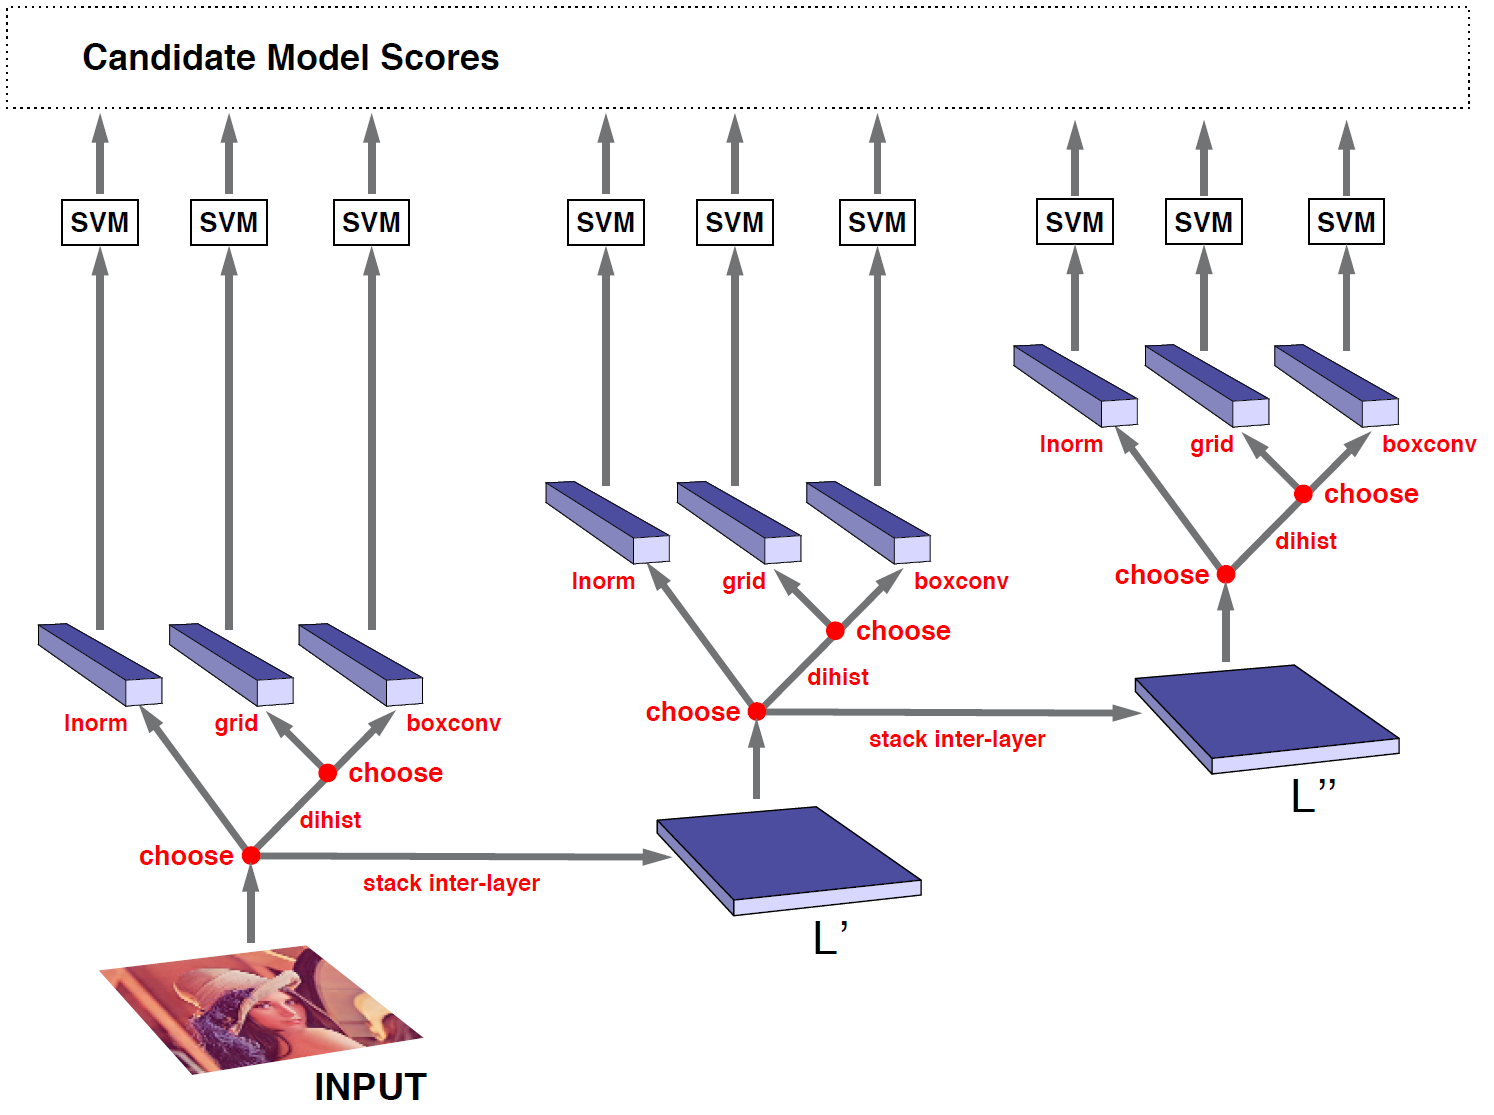
\includegraphics[width=.96\textwidth]{images/TPE_search_space.png}
\end{columns}
\pause


\begin{columns}
\column{0.00\textwidth}
\column{0.77\textwidth}
\vspace*{-0.4cm}
	\myit{
		\item With SMAC \lit{\href{https://ml.informatik.uni-freiburg.de/papers/11-LION5-SMAC.pdf}{Hutter et al. 2011}}:
		\myit{
			\item \alert{New state-of-the-art performance on CIFAR-10 w/o data augmentation} \lit{\href{https://ml.informatik.uni-freiburg.de/papers/15-IJCAI-Extrapolation_of_Learning_Curves.pdf}{Domhan et al. 2015}}
			\item Joint architecture and hyperparameter search, yielding Auto-Net \lit{\href{https://ml.informatik.uni-freiburg.de/papers/16-AUTOML-AutoNet.pdf}{Mendoza et al. 2016}}
\pause
			\item In 2015, Auto-Net already had several successes in ML competitions
			\myit{
				\item E.g., human action recognition:\\54491 data points, 5000 features, 18 classes 
				\item \alert{First automated deep learning (Auto-DL) method to win a machine learning competition dataset against human experts}
			}
		}
	}
\column{0.23\textwidth}
~\\~\\~\\~\\
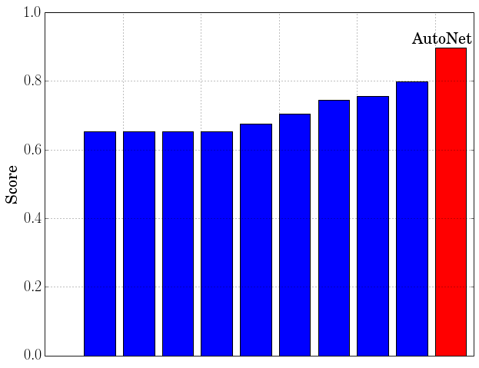
\includegraphics[width=.96\textwidth]{images/autonet-performance-competition.png}
\end{columns}

\pause
\smallskip

	\myit{
		\item With Gaussian processes: 
		\myit{
			\item Arc kernel \lit{\href{https://ml.informatik.uni-freiburg.de/papers/13-BayesOpt_Arc-Kernel.pdf}{Swersky et al. 2013}}
		}
	}
}




\myframe{Reinforcement Learning \litw{\href{https://arxiv.org/pdf/1611.01578.pdf}{Zoph and Le. 2016}}}{

{\begin{center}
	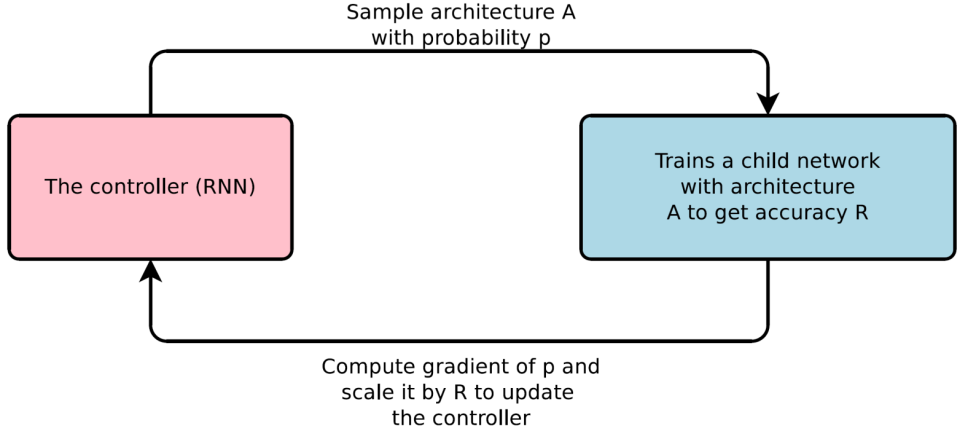
\includegraphics[width=.7\textwidth]{images/s27}
 \end{center}
}
\medskip
\begin{itemize}
	\item Use RNN (``\alert{Controller}'') to generate a NN architecture piece-by-piece
	\item Train this NN ("\alert{Child Network}") and evaluate it on a validation set
	\item Use \alert{Reinforcement Learning (RL)} to update the parameters of the Controller 
	RNN to optimize the performance of the child models
\end{itemize}

}
%----------------------------------------------------------------------

%----------------------------------------------------------------------
\myframe{Learning CNNs with RL \litw{\href{https://arxiv.org/pdf/1611.01578.pdf}{Zoph and Le. 2016}}}{

\centering
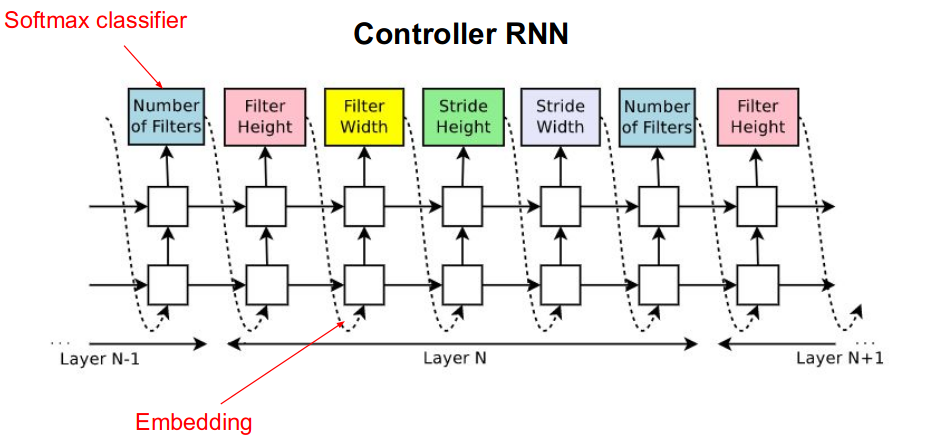
\includegraphics[width=.65\textwidth]{images/RL_CNN_controller}

\footnotesize{
	\myit{
	%	\item Maximize expected reward (validation accuracy): 
	%	$J(\theta_c)=E_{P(a_{1:T; \theta_c})}[R]$
		\item For a fixed number of layers, select:
		\begin{itemize}
			\item[-] \footnotesize Filter width/height, stride width/height, number of filters	
		\end{itemize}
	
	\pause
	\smallskip
		\item Large computational demands \alert{(800 GPUs for 2 weeks, 12.800 architectures evaluated)}
		%\myit{
		%	\item[-] \alert{800 GPUs for 2 weeks, 12.800 architectures evaluated}
		%}

	\pause
	\smallskip
	%	\item Each child model was trained for 50 epochs
	%	\item The final chosen architecture is trained for longer (600 epochs)
		%, optimizing the weights with SGD
		\item \alert{State-of-the-art results for CIFAR-10 \& Penn Treebank architecture}
		\myit{
			\item[$\rightarrow$] \footnotesize Brought NAS into the limelight
		}
	}
	}
}
%----------------------------------------------------------------------

%----------------------------------------------------------------------

\myframetop{Learning CNN cells with RL \litw{\href{https://openaccess.thecvf.com/content_cvpr_2018/papers/Zoph_Learning_Transferable_Architectures_CVPR_2018_paper.pdf}{Zoph et al. 2018}}}{
	\centering
	
	\begin{itemize}
		\item 2 types of cells: normal and reduction cells
		\item For each type of cell: $B$ blocks, each with 5 choices
		\myit{
			\item[-] Choose two previous feature maps (from this cell)
			\item[-] For each of these, choose an operation (3$\times$3 conv, max-pool, etc.)
			\item[-] Choose a merge operation to combine the two results (concat or add)
		}
	
	\end{itemize}
	\bigskip
	\bigskip
	\smallskip
	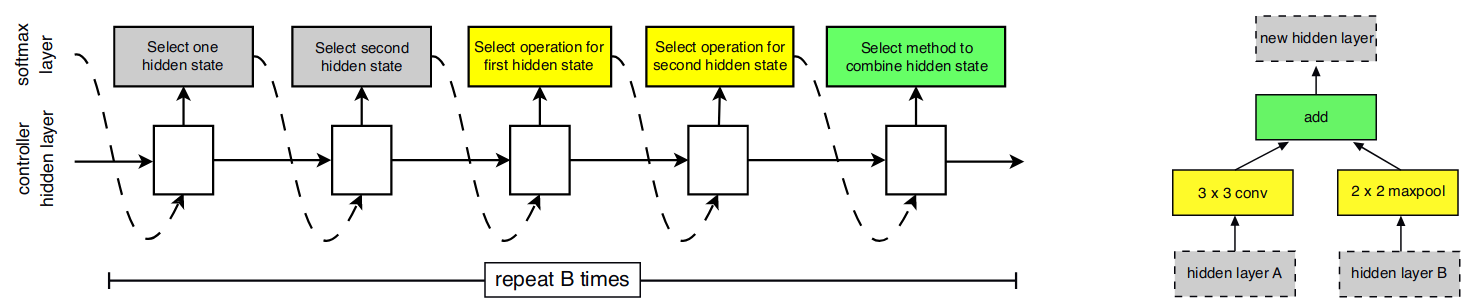
\includegraphics[width=\textwidth]{images/RL_conv_cell}
	%\pause
	%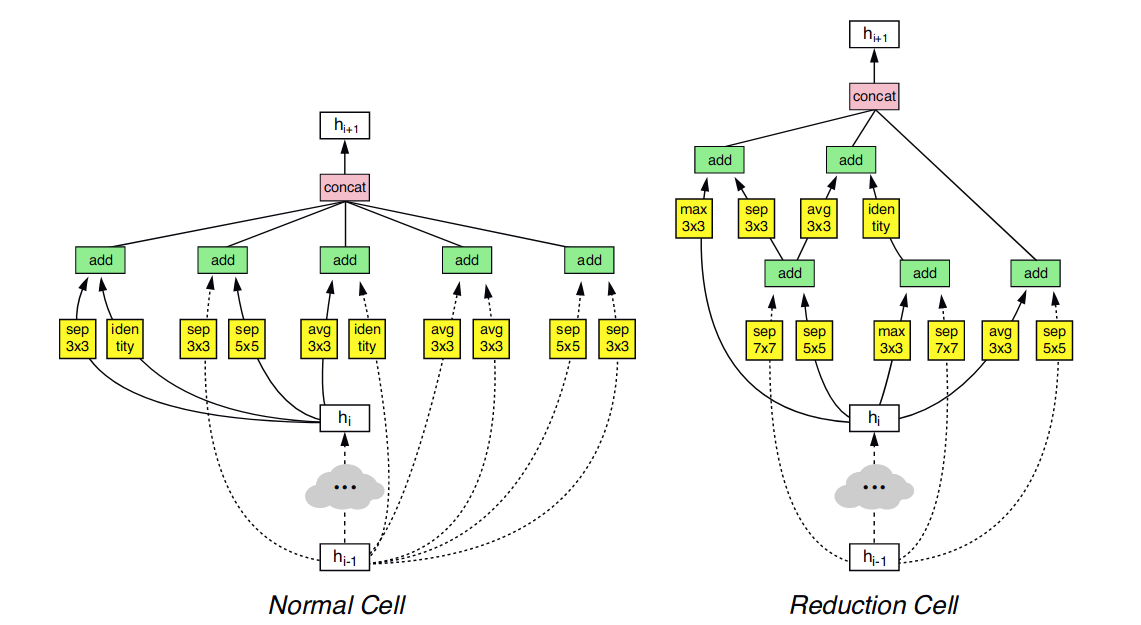
\includegraphics[width=.5\textwidth]{images/RL_normal_reduction}
	
}
%----------------------------------------------------------------------
%----------------------------------------------------------------------

\myframetop{Learning CNN cells with evolution \litw{\href{https://arxiv.org/pdf/1802.01548.pdf}{Real et al. 2018}}}{
	\begin{itemize}
		\item 2 types of cells: normal and reduction cells
		\item For each type of cell: $B$ blocks, each with 5 choices
		\myit{
			\item[-] Choose two previous feature maps (from this cell)
			\item[-] For each of these, choose an operation (3$\times$3 conv, max-pool, etc.)
			\item[-] Choose a merge operation to combine the two results (concat or add)
		}
	
	\end{itemize}
	\bigskip
	
	\begin{itemize}
	  \item Evolution simply tackles this as a HPO problem with 2$\times$5$\times$B variables:
	\end{itemize}
	~~~~~~~~\vspace*{0.20cm}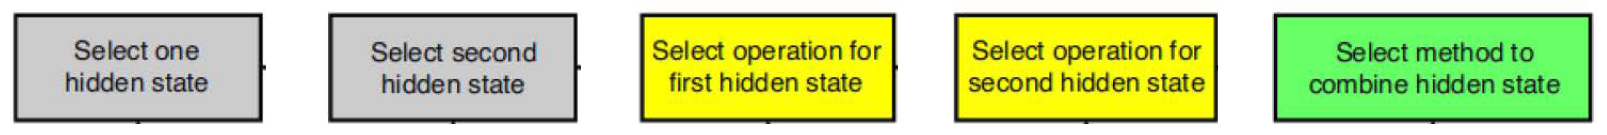
\includegraphics[width=0.616\textwidth]{images/NAS-RL-space_as_HPO}
	
}

%----------------------------------------------------------------------
%----------------------------------------------------------------------

%\myframe{Evolution}{
%
%\centering
%\begin{enumerate}
%	\footnotesize
%	\item Initialize a \alert{population} of randomly sampled architectures.
%	\item Sample pairs and select the architecture to mutate based on the \emph{fitness} function (e.g. validation error). \alert{Remove} the other from the population.
%	\item Apply \alert{mutation} steps to the selected architecture, such as adding, changing or removing a layer. Add the new child architecture to the population. \lit{\href{https://arxiv.org/abs/1703.01041}{Real et al. 2017}; \href{https://openreview.net/forum?id=BJQRKzbA-}{Liu et al. 2017}; \href{https://arxiv.org/pdf/1703.00548.pdf}{Miikkulainen et al. 2017}}
%\end{enumerate}
%
%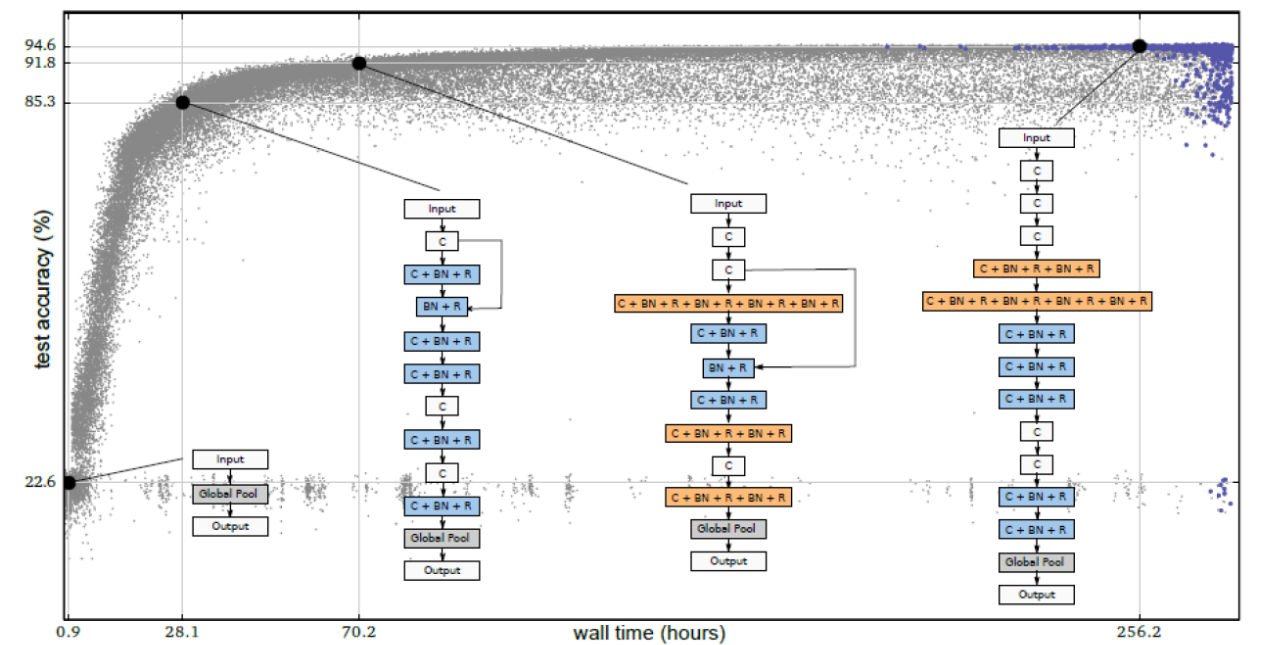
\includegraphics[width=.7\textwidth]{images/neuroevolution.png}\\
%}
% Narrative: One approach that has been used to search in such NAS spaces is Neuroevolution. This has already been studied since the 1990s in the Neuroevolution literature. Typically, it optimized both the architecture and the weights of the neural network with evolutionary methods. For example, it used a mutation step, such as adding layers or changing a layer or removing a layer. In this visualization here, you can see that you start with a pretty simple network and then over time the network gets more complicated and at the end you actually get a fairly complicated and well performing model. In the meantime, people have realized that for optimizing the weights of the neural network, the evolutionary methods are not typically competitive. If you have supervised learning and you have clean gradients, then to optimize in the space of potentially millions of different weights, stochastic gradient descent is just far better than evolutionary methods. So nowadays, the typical evolution methods would only use evolution for the architecture and not for the weights. For the weights, you would use the same type of black-box optimization that has been used for RL.

%----------------------------------------------------------------------

%----------------------------------------------------------------------
\myframe{Regularized/Aging Evolution \litw{\href{https://arxiv.org/pdf/1802.01548.pdf}{Real et al. 2018}}}{

\centering
\begin{itemize}
	\item Quite standard evolutionary algorithm
	\myit{
		\item But oldest solutions are dropped from population, instead of the worst
	}
\pause
	\item Standard SGD for training weights (\alert{optimizing the same blackbox as RL})
	\item \alert{Same fixed-length (HPO) search space} as used for RL \lit{\href{http://openaccess.thecvf.com/content_cvpr_2018/html/Zoph_Learning_Transferable_Architectures_CVPR_2018_paper.html}{Zoph et al. 2018}}
\end{itemize}

\bigskip
\begin{columns}[T]

\column{0.36\textwidth}
\centering
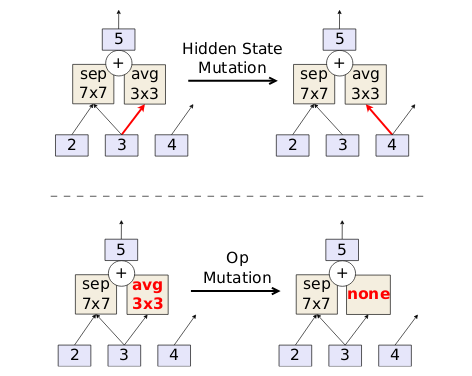
\includegraphics[width=\textwidth]{images/aging_evolution_mutations.png}
\footnotesize{Different types of mutations in cell search space}
\pause
\column{0.36\textwidth}
\centering
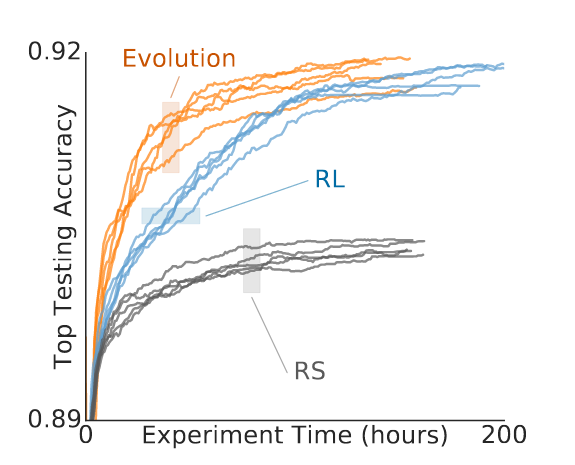
\includegraphics[width=.9\textwidth]{images/aging_evolution_results.png}
\footnotesize{\alert{State-of-the-art performance in apples-to-apples comparison}\\ $\rightarrow$ \alert{AmoebaNet}}
\end{columns}

}
%----------------------------------------------------------------------

%----------------------------------------------------------------------
\myframe{Bayesian Optimization (BO)}{
	\myit{
		\item Encode the architecture space by categorical hyperparameters (like regularized evolution)
\medskip
		\item \alert{Strong performance with tree-based models} 
		\myit{
			\item TPE \lit{\href{http://proceedings.mlr.press/v28/bergstra13.pdf}{Bergstra et al. 2013}}
			\item SMAC \lit{\href{https://ml.informatik.uni-freiburg.de/papers/15-IJCAI-Extrapolation_of_Learning_Curves.pdf}{Domhan et al. 2015}; \href{https://ml.informatik.uni-freiburg.de/papers/16-AUTOML-AutoNet.pdf}{Mendoza et al. 2016}; \href{https://arxiv.org/pdf/1807.06906.pdf}{Zela et al. 2018}}
		}
	}

\pause
\medskip
	\myit{
		\item Kernels for GP-based NAS
		\myit{
			\item[-] Arc kernel \lit{\href{https://ml.informatik.uni-freiburg.de/papers/13-BayesOpt_Arc-Kernel.pdf}{Swersky et al. 2013}}
			\item[-] NASBOT \lit{\href{https://arxiv.org/pdf/1802.07191.pdf}{Kandasamy et al. 2018}}
		}
\pause
\medskip		

		\item There are also several recent promising BO approaches based on neural networks
		\myit{
			\item[-] BANANAS \lit{\href{https://arxiv.org/pdf/1910.11858.pdf}{White et al. 2019}}
		}
\pause
\medskip
		\item BO is very competitive, has been shown to outperform RL \lit{\href{https://arxiv.org/pdf/1902.09635.pdf}{Ying et al. 2019}}
	}
}
%-----------------------------------------------------------------------


%----------------------------------------------------------------------
\myframe{Current State of the Art: Differential Evolution}{
	\myit{
		\item Comprehensive experiments on a wide range of 12 different NAS benchmarks\\
		\lit{\href{https://drive.google.com/file/d/1kxhLeXnwiAkarkXU15GrU3vyodKETWQw/view?usp=sharing}{Awad et al. 2020}} 
\bigskip
\pause
		\item Results:
		\myit{
			\item \alert{Regularized evolution is very robust}, typically amongst best of the methods discussed so far
			\item Evolution variant of \alert{differential evolution is yet better}; most efficient and robust method
		}
	}	 
\begin{center}
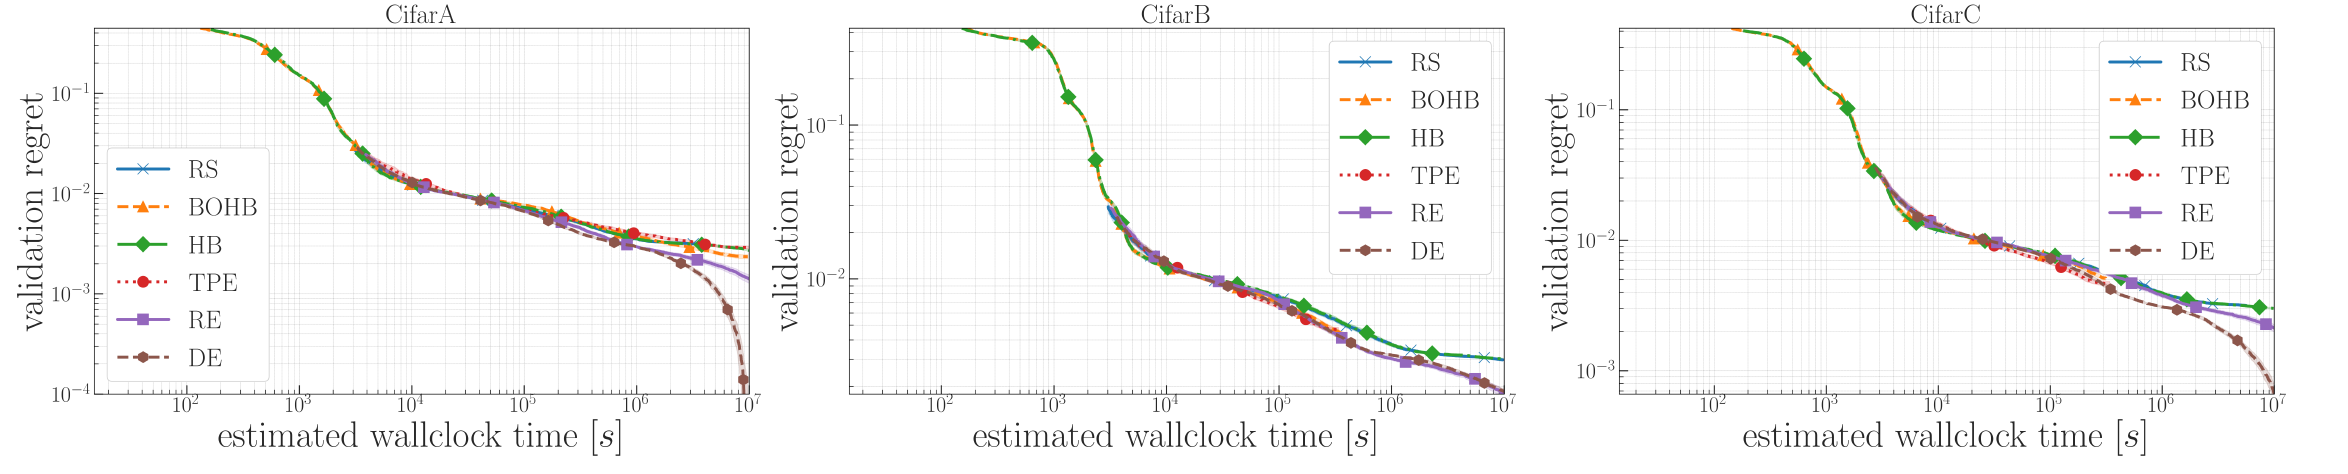
\includegraphics[width=.9\textwidth]{images/DE_results_NB101.png}
\end{center}	
	
%	\myit{
%		\item Possible explanation: quite greedy method, locality in the search space
%	}
}
%-----------------------------------------------------------------------


%----------------------------------------------------------------------
%\myframe{Case study: NASBOT \litw{\href{https://arxiv.org/abs/1802.07191}{Kandasamy et al., NeurIPS 2018}}}{
%
%\centering
%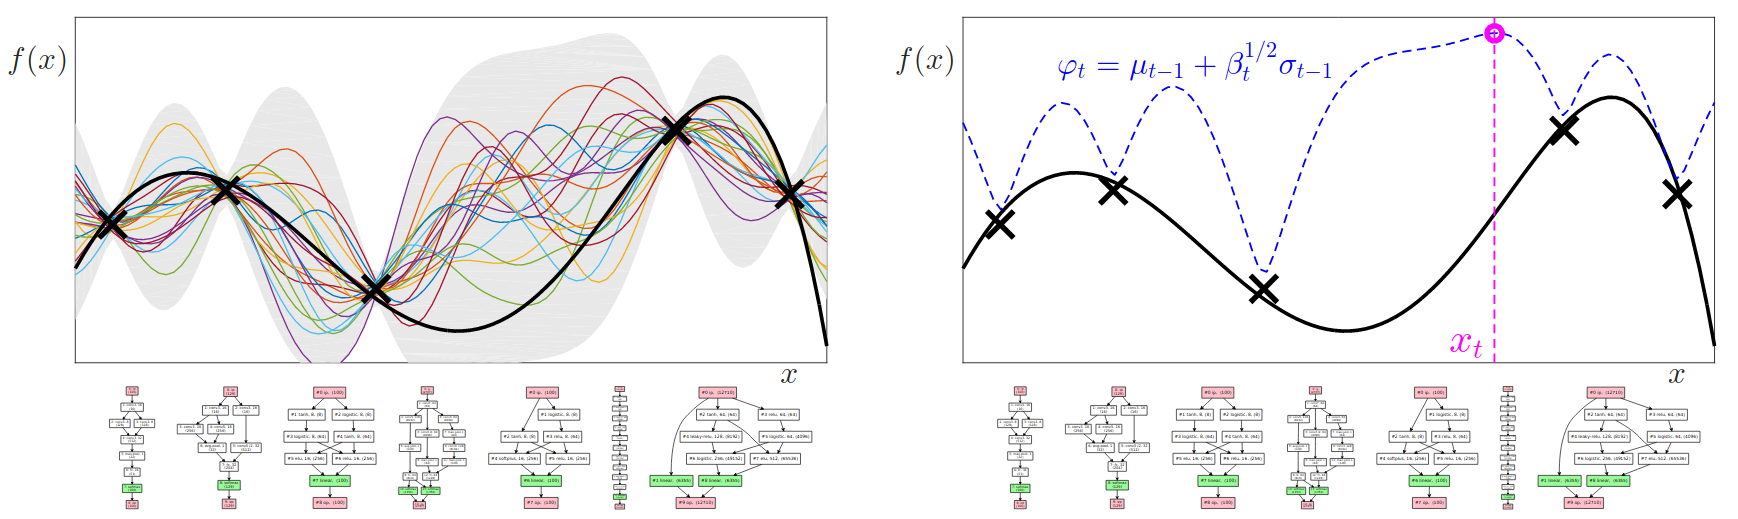
\includegraphics[width=.9\textwidth]{images/nasbot_1.png}
%\myit{
%\footnotesize
%		\item Gaussian Process BO is not that straighforward in non-Euclidian spaces such as the space of neural architectures
%		\myit{
%		\footnotesize
%			\item How to define a kernel (which entails the distance) in the architecture space?
%			\item How to optimize the acquisition function?
%		}
%\pause
%\medskip
%		\item \alert{NASBOT}
%		\myit{
%		\footnotesize
%			\item defines a distance metric based on Optimal Transport (\alert{OTMANN})
%			\item optimizes the acquisition function using \alert{evolution}
%		}		
%}
%
%}
%
%%----------------------------------------------------------------------
%\myframe{Case study: NASBOT \litw{\href{https://arxiv.org/abs/1802.07191}{Kandasamy et al., NeurIPS 2018}}}{
%
%\centering
%
%\begin{columns}
%\column{.6\textwidth}
%\vspace{-7cm}
%\myit{
%		\item The kernel: $\kappa = e^{-\beta d^{p}}$, where $d$ is the OTMANN distance
%		\myit{
%			\item[--] To compute $d$ between two architectures $G_1$, $G_2$: match computation (layer mass) in layers in $G_1$ to $G_2$
%		}
%}
%\pause
%\medskip
%
%\myit{
%	\item $Z \in \mathtt{R}^{n_1 \times n_2}$
%	\myit{
%		\item $Z_{ij} \longleftarrow$ \alert{amount of matched mass} between layer $i\in G_1$ and $j \in G_2$
%	}
%	\medskip
%	\item $d \triangleq \argminA_Z \phi_{lmm}(Z) + \phi_{str}(Z) + \phi_{nas}(Z)$
%	\myit{
%		\item[--] $\phi_{lmm}(Z)$: label mismatch penalty
%		\item[--] $\phi_{str}(Z)$: structural penalty
%		\item[--] $\phi_{nas}(Z)$: non-assignment penalty
%	}
%}
%
%\column{.4\textwidth}
%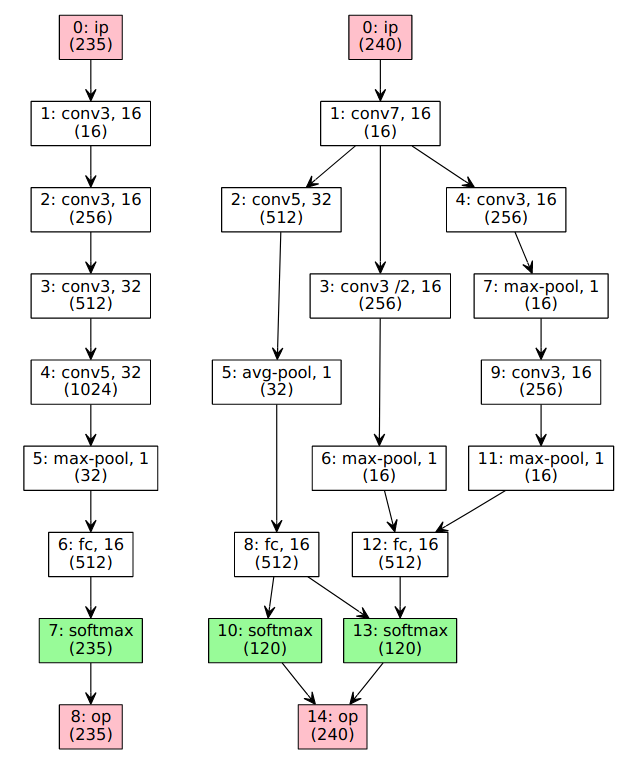
\includegraphics[width=\textwidth]{images/nasbot_2.png}
%
%\end{columns}
%
%}
%%-----------------------------------------------------------------------

%----------------------------------------------------------------------
\myframe{Questions to Answer for Yourself / Discuss with Friends}{

	\myit{
		\item Repetition:\\ 
		\alert{What are some pros and cons of using black-box optimizers for NAS?}
\medskip
		\item Repetition:\\
		\alert{How can NAS be modelled as a HPO problem?}
		%\item Repetition: \alert{Which blackbox NAS approach popularized the field?}
%\medskip
%		\item Repetition: \alert{Which blackbox NAS approach works best (to date)?}
\medskip
		\item Discussion:\\ \alert{Given enough resources, will blackbox NAS approaches always improve performance?}
\medskip
		\item Discussion:\\ \alert{Why does discarding the oldest individual (rather than the worst) help in regularized/aging evolution?}
\medskip
		\item Transfer:\\ 
		\alert{How would you write NAS with the hierarchical search space as a HPO problem?}
	}	 
}
%-----------------------------------------------------------------------

